\begin{frame}{Potential Problems}

When we fit a linear regression model to a particular data set, many problems may occur. Most common among these are the following:

%%%%%%%%%%%%%%%%%%%%%%%% OUTLINE %%%%%%%%%%%%%%%%%%%%%%%%%%%%%%

\begin{enumerate}
    \item<1-2> Non-linearity of the response-predictor relationships.
    \item<1> Correlation of error terms.
    \item<1> Non-constant variance of error terms.
    \item<1> Outliers.
    \item<1> High-leverage points.
    \item<1> Collinearity.
\end{enumerate}
    
\end{frame}

\begin{frame}{Potential Problems}{Non-linearity of the Data}

    
\begin{itemize}
    \item The linear regression model assumes that there is a straight-line relationship between the predictors and the response. \pause
    
    \item If the true relationship is far from linear, then virtually all of the conclusions that we draw from the fit are suspect. \pause

    \item \textit{Residual plots} are a useful graphical tool for identifying non-linearity. 

    \item In the case of a multiple regression model, we plot the residuals versus the predicted (or fitted) values $\hat{y}_i$. 


    \end{itemize}

\end{frame}

\begin{frame}{Potential Problems}{Non-linearity of the Data}

\begin{itemize}
    \item Ideally, the residual plot will show no fitted discernible pattern. \pause

    \item The presence of a pattern may indicate a problem with some aspect of the linear model. \pause
\end{itemize}

\begin{columns}

    \column{0.4\linewidth}    
    \begin{figure}[!h]
        \centering
        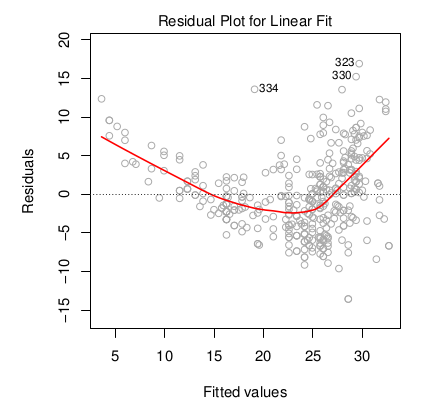
\includegraphics[height=4cm, width=4cm]{other-lr/residual_fit.png}
    \end{figure} \pause

    \column{0.4\linewidth}    

    \begin{block}{Note}
    If the residual plot indicates that there are non-linear associations in the data, then a simple approach is to use \textbf{non-linear transformations} of the predictors, such as log$X$ and $\sqrt{X}$, in the regression model. 
    \end{block}
    
    
\end{columns}
    
\end{frame}    

%%%%%%%%%%%%%%%%%%%%%%%% OUTLINE %%%%%%%%%%%%%%%%%%%%%%%%%%%%%%

\begin{frame}[noframenumbering]{Potential Problems}


\begin{enumerate}
    \item<1> Non-linearity of the response-predictor relationships.
    \item<1-2> Correlation of error terms.
    \item<1> Non-constant variance of error terms.
    \item<1> Outliers.
    \item<1> High-leverage points.
    \item<1> Collinearity.
\end{enumerate}
    
\end{frame}

\begin{frame}{Potential Problems}{Correlation of Error Terms}

\begin{itemize}
    \item An important assumption of the linear regression model is that the error terms, $\epsilon_1, \epsilon_2, \cdots, \epsilon_n$, are uncorrelated. \pause \\
    $\rightarrow$ i.e. the fact that $\epsilon_i$ is positive provides little or no information about the sign of $\epsilon_{i+1}$. \pause

    \item Is there is correlation among the error terms, then the estimated standard errors will tend to underestimate the true standard errors. \pause
    
    \item As a result, confidence and prediction intervals will be narrower than they should be. \pause

    \item In addition, p-values associated with the model will be lower than they should be; this could cause us to erroneously conclude that a parameter is statistically significant. \pause

    \item Why might correlations among the error terms occur? \pause \\ $\rightarrow$ Such correlations frequently occur in the context of \textbf{time series data}.
    
\end{itemize}


\end{frame}

\begin{frame}{Potential Problems}{Correlation of Error Terms}

\begin{itemize}
    \item In order to determine if this is the case for a given data set, we can plot the residuals from our model as a function of time. \pause

    \item If the errors are \textcolor{blue}{uncorrelated}, then there should be \textcolor{blue}{no discernible pattern}. \pause

    \item If the error terms are \textcolor{blue}{positively correlated}, then we may see \textcolor{blue}{tracking} in the residuals. \pause $\rightarrow$ adjacent residuals may have similar values. \pause

    
    \begin{figure}[!h]
    \centering
    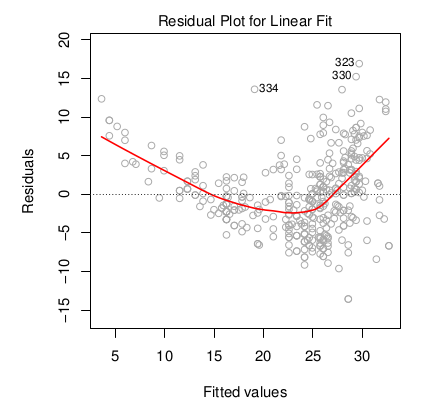
\includegraphics[height=4cm, width=7.5cm]{other-lr/residual_fit.png}
    \end{figure} \pause
    \item Good experimental design is crucial in order to mitigate the risk of such correlations.
    
\end{itemize}

    
\end{frame}


\begin{frame}[noframenumbering]{Potential Problems}


\begin{enumerate}
    \item<1> Non-linearity of the response-predictor relationships.
    \item<1> Correlation of error terms.
    \item<1-2> Non-constant variance of error terms.
    \item<1> Outliers.
    \item<1> High-leverage points.
    \item<1> Collinearity.
\end{enumerate}
    
\end{frame}

\begin{frame}{Potential Problems}{Non-constant Variance of Error Terms}

\begin{itemize}
    \item Another important assumption of the linear regression model is that the error terms have a constant variance, $Var(\epsilon_i ) = \sigma^2$ \pause

    \item One can identify non-constant variances in the errors, or \textcolor{blue}{heteroscedasticity}, from the presence of a funnel shape in the residual plot. \pause

    \item When faced with this problem, one possible solution is to transform the response $Y$ using a \textbf{concave} function  such as $log(Y)$ or $\sqrt{Y}$. \pause

    \item Such a transformation results in a greater amount of shrinkage of the larger responses, leading to a reduction in heteroscedasticity. \pause

\end{itemize}
    
\end{frame}

\begin{frame}{Potential Problems}{Non-constant Variance of Error Terms}

    \begin{figure}[!h]
    \centering
    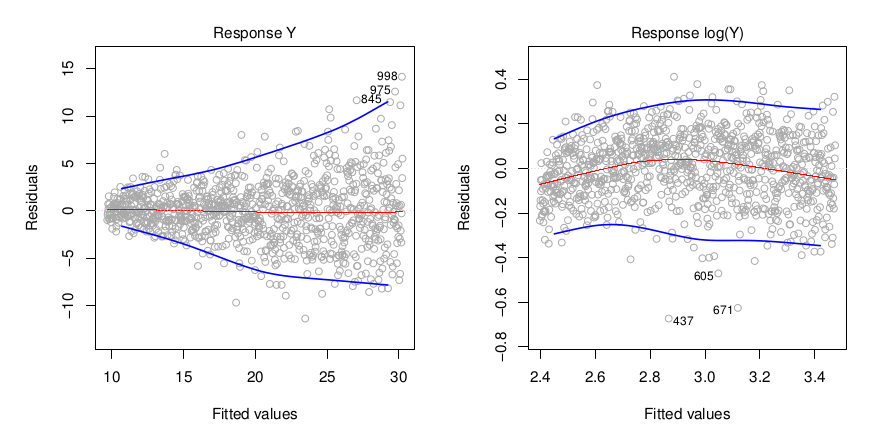
\includegraphics[height=6cm, width=9.5cm]{other-lr/heteroscedasticity.png}
    \end{figure} 
    
\end{frame}


\begin{frame}[noframenumbering]{Potential Problems}


\begin{enumerate}
    \item<1> Non-linearity of the response-predictor relationships.
    \item<1> Correlation of error terms.
    \item<1> Non-constant variance of error terms.
    \item<1-2> Outliers.
    \item<1> High-leverage points.
    \item<1> Collinearity.
\end{enumerate}
    
\end{frame}

\begin{frame}{Potential Problems}{Outliers}

    \begin{itemize}
        \item An outlier is a point for which $yi$ is far from the value predicted by the outlier model. \pause

        \item Include outliers in the regression fit can cause alterations on the RSE values, which are further used to compute confidence intervals and p-values. \pause

        \item A single data point can have implications for the interpretation of the fit. \pause

        \item To identify outliers, we can compute the \textbf{studentized residuals} by dividing each residual $e_i$ by its estimated standard error. \pause

        \item Observations whose studentized residuals are greater than 3 in absolute value are possible outliers. \pause
        
    \end{itemize}

\end{frame}

\begin{frame}{Potential Problems}{Outliers}
    \begin{figure}
        \centering
        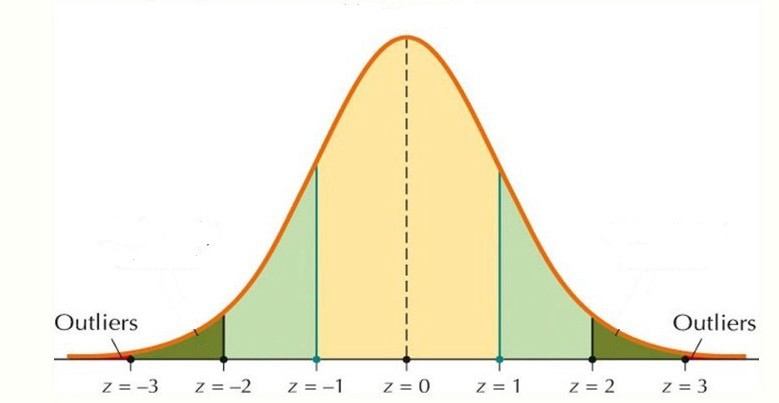
\includegraphics[height=5cm, width=8.5cm]{other-lr/outlier.jpeg}
    \end{figure}

    \begin{block}{Notes}
        \begin{itemize}
            \item If we believe that an outlier has occurred due to an error in data collection or recording, then one solution is to simply remove the observation. \pause
            \item However, care should be taken, since an outlier may instead indicate a deficiency with the model, such as a missing predictor.
    \end{itemize}            
    \end{block}
\end{frame}


%%%%%%%%%%%%%%%%%%%% OUTLINE %%%%%%%%%%%%%%%%%%%%%%%%
\begin{frame}[noframenumbering]{Potential Problems}


\begin{enumerate}
    \item<1> Non-linearity of the response-predictor relationships.
    \item<1> Correlation of error terms.
    \item<1> Non-constant variance of error terms.
    \item<1> Outliers.
    \item<1-2> High-leverage points.
    \item<1> Collinearity.
\end{enumerate}
    
\end{frame}

\begin{frame}{Potential Problems}{Outliers}

\begin{itemize}
    \item We just saw that outliers are observations for which the response $y_i$ is unusual given the predictor $x_i$. \pause 
    
    \item In contrast, observations with \textbf{high leverage} have an \textbf{unusual value for $x_i$}. \pause
    
    \item High leverage observations tend to have a sizable impact on the estimated regression line. \pause
    
    \item In order to quantify an observation’s leverage, we compute the \textcolor{blue}{leverage statistic}: \pause

    $$h_i = \frac{1}{n} + \frac{(x_i - \Bar{x})^2}{\sum_{i'=1}^n (x_i' - \Bar{x})^2 }$$ \pause

    \end{itemize}
    \end{frame}

\begin{frame}{Potential Problems}{Outliers}

$$h_i = \frac{1}{n} + \frac{(x_i - \Bar{x})^2}{\sum_{i'=1}^n (x_i' - \Bar{x})^2 }$$ \pause

\begin{itemize}

    \item A large value of this statistic indicates an observation with high leverage.
    
\end{itemize}

\begin{block}{Notes}
    $\rightarrow$ $h_i$ increases with the distance of $x_i$ from $\Bar{x}$. \pause  \\

    $\rightarrow$ The average leverage for all the observations is always equal to $(p + 1)/n$. \pause \\
    
    $\rightarrow$ If a given observation has a leverage statistic that greatly exceeds $(p+1)/n$, then we may suspect that the corresponding point has high leverage.   
\end{block}
    
    
\end{frame}


\begin{frame}[noframenumbering]{Potential Problems}


\begin{enumerate}
    \item<1> Non-linearity of the response-predictor relationships.
    \item<1> Correlation of error terms.
    \item<1> Non-constant variance of error terms.
    \item<1> Outliers.
    \item<1> High-leverage points.
    \item<1-2> Collinearity.
\end{enumerate}
    
\end{frame}

\begin{frame}{Potential Problems}{Collinearity}

    \begin{itemize}
        \item Collinearity refers to the situation in which two or more predictor variables collinearity are closely related to one another. \pause

        \item The presence of collinearity can pose problems in the regression context, since it can be difficult to separate out the individual effects of collinear variables on the response. \pause

        \item Collinearity reduces the accuracy of the estimates of the regression coefficients, it causes the standard error for $\hat{\beta}_j$ to grow. \pause
        \item Recall that the \textit{t-statistic} for each predictor is calculated by dividing $\hat{\beta_j}$ by its standard error. \pause
        
        \item Consequently, collinearity results in a decline in the t-statistic. As a result, in the presence of collinearity, we may fail to reject $H_0 : \beta_j = 0 $.

    \end{itemize}
    
    
\end{frame}


\begin{frame}{Potential Problems}{Collinearity}

\textbf{How to detect collinearity (or multicollinearity):}

\begin{itemize}
    \item Look at the \textcolor{blue}{correlation matrix} of the predictors. \pause \\ 
    $\rightarrow$ An element of this matrix that is large in absolute value indicates a pair of highly correlated variables. \pause

    \item Compute the \textcolor{blue}{variance inflation factor (VIF)}. \pause \\
    $\rightarrow$ The VIF is the ratio of the variance of $\hat{\beta}_j$ when fitting the \textit{full model} divided by the variance of $\hat{\beta}_j$ if fit on \textit{its own}. \pause

    $$ VIF(\hat{\beta}_j) = \frac{1}{1- R^2_{Xj|X_{-j}}}, $$ \pause
    where $R^2_{Xj|X_{-j}}$ is the $R^2$ from a regression of $X_j$ onto all of the other predictors.

    \end{itemize}
    
\end{frame}

\begin{frame}{Potential Problems}{Collinearity}
    $$ VIF(\hat{\beta}_j) = \frac{1}{1- R^2_{Xj|X_{-j}}}, $$
    where $R^2_{Xj|X_{-j}}$ is the $R^2$ from a regression of $X_j$ onto all of the other predictors. \pause

    \begin{itemize}
        \item If $VIF \simeq$ 1 $\rightarrow$  complete absence of collinearity. \pause
        \item If $1 < VIF < 5$ $\rightarrow$  moderate collinearity. \pause
        \item If $VIF > 5$ $\rightarrow$  high collinearity. \pause
    \end{itemize}

\textbf{Solutions:} \pause
    \begin{enumerate}
        \item Drop one of the problematic variables from the regression. \pause 
        \item Combine the collinear variables together into a single predictor. 
    \end{enumerate}

    
\end{frame}


    
